\subsection{Studying ignored bounty issue reports}
\label{rq4}

%\noindent\textbf{Motivation:}
%\sw{update later}
In Section~\ref{prestudy}, we observed that in 19.7\% of the bounty issue reports the bounties were ignored (i.e., closed-unpaid). For these ignored bounty issue reports, the issue reports were closed but the bounties remained unclaimed.
It seems that money was not the driver that motivated developers to address these issues.
To understand the possible reasons behind this phenomenon, we manually studied all 692 ignored bounty issue reports (with a total bounty value of \$41,856).
Because the ``closed'' status of an issue report does not necessarily mean that the issue was addressed (e.g., a report may have been a duplicate of another issue report), it is very difficult to automatically identify whether an issue in the closed issue report was addressed or not.
Therefore, we need to manually examine the closed-unpaid bounty issues reports to filter out the reports that were closed for another reason than the issue being addressed.

%The first two authors independently manually examined these reports and their corresponding discussion to decide whether these particular reports were addressed. Discrepancies were discussed by the two authors until a consensus was reached. We use Cohen's kappa~\cite{cohenkappa} to measure the inter-rater agreement and the value was 0.86, which is considered as an almost perfect agreement \cite{landis1977measurement}. During the examination, the authors also searched for comments that gave an explicit reason as to why no developer claimed the bounty.

%\begin{figure}[t]
%\centering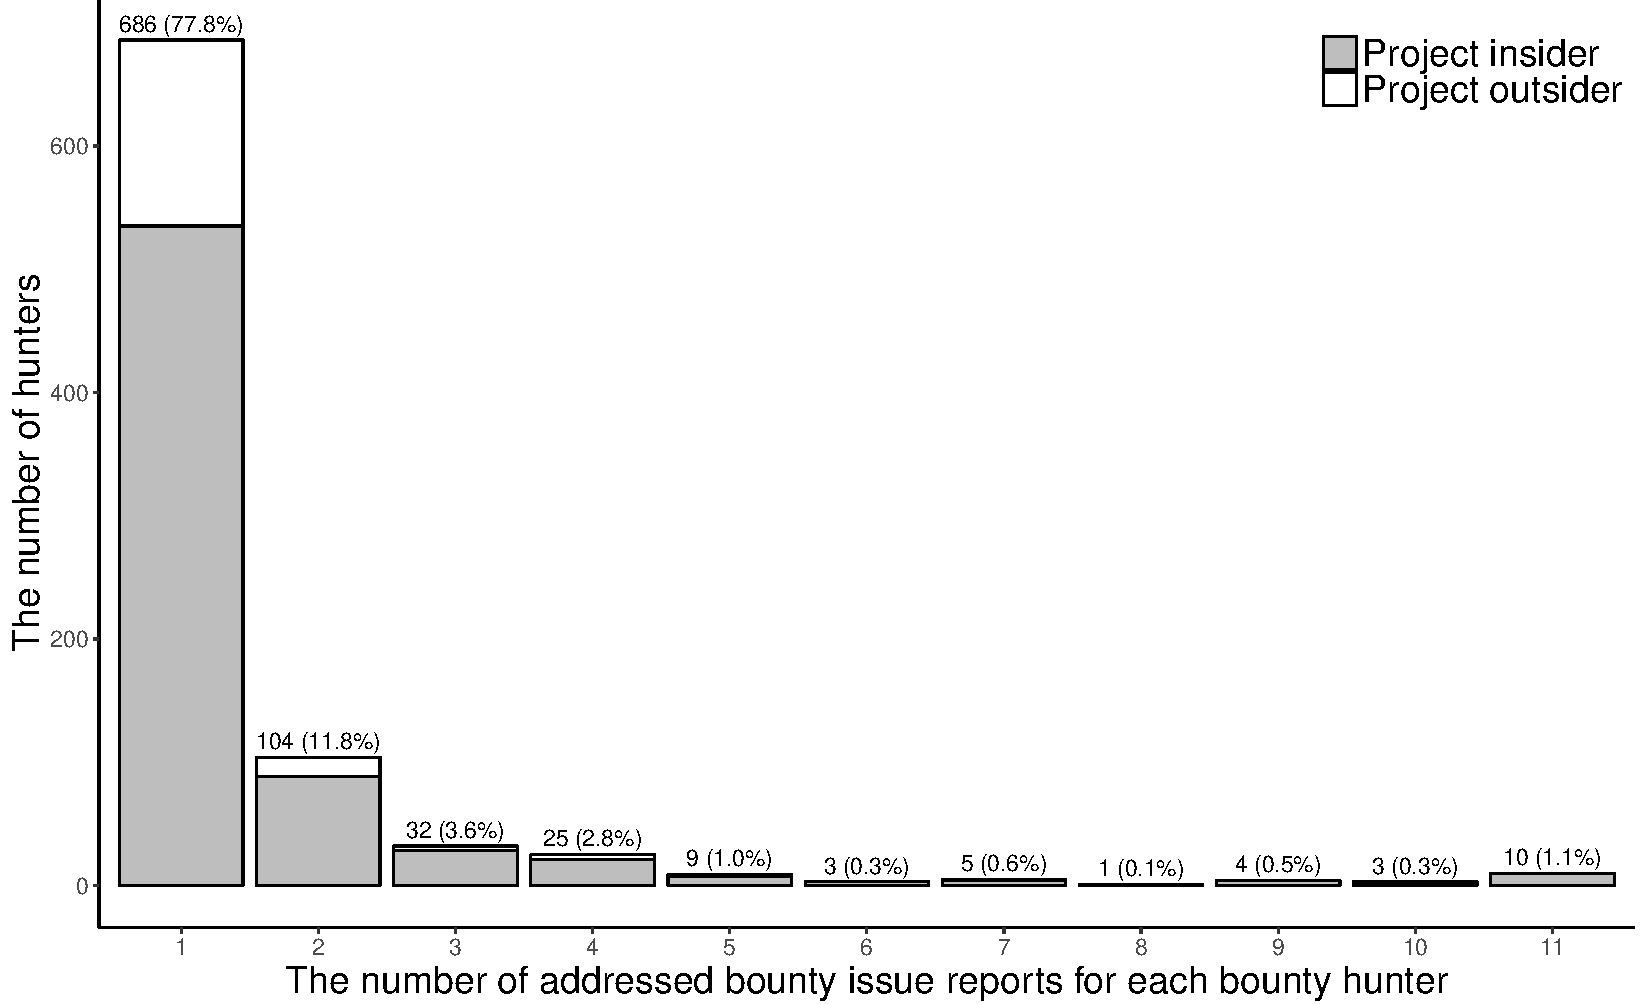
\includegraphics[width=\columnwidth]{pics/rq2/newrq2_distribution_hunter_issue_cnt.pdf}
%  \caption{The number and proportion (presented at the top of each bar) of hunters that addressed x bounty issue reports in the past.  }
%  \label{hunter_isseu_cnt}
%\end{figure}


%479/(479+1508)
\textbf{21.8\% (479 out of 2,200) of the addressed bounty issue reports were not paid out.} We identified that 479 out of the studied 692 bounty issue reports were closed because the issues were addressed. Such cases are interesting since the developers could have claimed the bounty but they did not. We manually examined the discussion for these 479 issue reports. We identified 19 cases in which developers gave an explanation for not claiming the bounty. We grouped the explanations as follows:

\noindent\textbf{The developer is not driven by money.} In 7 out of 19 cases a developer refused to claim the bounty because they were not motivated by money to address the issue.
For example, one developer was against the bounty because they felt that the issue-addressing process should be driven by the interests of the community rather than money. A contributor of the \code{Brython} project,%\footnote{\url{https://brython.info/}}
 refused the bounty because he wanted to keep \code{Brython} free from monetary motivations: ``\textit{What is this `bounty' thing? Needless to say, I refuse that anybody (me included, of course) gets paid for anything related to \code{Brython}.}''\footnote{\url{%https://github.com/brython-dev/brython/issues/680\#issuecomment-330474874
http://bit.ly/2OTYx0x}} In addition, he also asked bounty backers to remove all bounties within the \code{Brython} project although he respected prior bounties that were paid out. There were five bounty issue reports in the \code{Brython} project and four bounty issue reports that were addressed without claiming the bounty.

%Similarly to the \code{Brython} project, the owner of the \code{Pi-hole} project\footnote{\url{https://pi-hole.net/}}, shut down\footnote{\url{https://github.com/pi-hole/pi-hole/issues/371\#issuecomment-379938463}} the usage of the bounty within \code{Pi-hole} because he believed \code{Pi-hole} should be driven by the community need instead of money.
%The developers refused to receive bounties directly since they think that financial incentive should not be involved in open source projects.

\noindent\textbf{The developer is afraid of sending the wrong message.} Krishnamurthy et al. \cite{krishnamurthy2006bounty} pointed out that financial incentives may cause confusion in the community because the financial incentives may drive a project's own product development cycle away from what is in place.
We observed that developers expressed similar concerns. A developer of the \code{Facebook/HHVM} project,%\footnote{\url{https://hhvm.com/}}
 explained that: ``\emph{That's very generous of you, but I can't accept a bounty for doing my job. :-P It would be a conflict of interest, and I worry it sends the wrong message about how we prioritize issues from the community.}''\footnote{\url{%https://github.com/facebook/hhvm/issues/1203\#issuecomment-55794203
http://bit.ly/2OZw1uw}}

%In another example, a developer of the \code{OSVR} project\footnote{\url{http://www.osvr.org/}} refused to claim the bounty and explained: ``\textit{I've already been paid for my part in this code, so I'm happy to see the bounty distributed to the others.}''




\noindent\textbf{The issue report was addressed by more than one developer.} We found nine cases where bounties ended up unclaimed because an issue report was addressed by multiple developers cooperatively and they felt inappropriate to claim the bounty by one developer. For example, the issue\footnote{\url{%https://github.com/numixproject/numix-icon-theme/issues/450/\#issuecomment-143499209
http://bit.ly/2PrMiHV}} was addressed by two developers and because a bounty cannot be split into two parts, no one claimed it.





\subsection{The implications of our findings}
\textbf{Backers should consider proposing a bounty as early as possible and be cautious when proposing small bounties on long-standing issue reports.}
The timing of proposing a bounty is an important factor that impacts the issue-addressing likelihood. In Sections~\ref{rq2} and~\ref{rq3}, we revealed the fact that issue reports for which bounties were proposed earlier are more likely to be addressed. Additionally, we observed that issue reports for which bounties were proposed earlier are more likely to be addressed faster. Backers benefit from the higher issue-addressing likelihood and faster issue-addressing speed by proposing bounties earlier.

In Section~\ref{rq2}, we also noticed a big drop (i.e., from 53.2\% to 30.1\%) of the issue-addressing likelihood when backers proposed bounties on long-standing (i.e., more than half a year) issue reports. This drop might be due to such issue reports having become obsolete or being hard to address.
Since bounties with a value of less than \$100 will not be refunded to the backers if the issue report remains unaddressed, we suggest that backers be cautious when proposing small bounties on long-standing issue reports.

\textbf{Backers should consider proposing a relatively bigger bounty in first-timer bounty-projects.} %In %Section~\ref{rq1}, we observed a positive relationship between the issue-addressing likelihood and the bounty-usage frequency. The global models in Section~\ref{rq3} also show similar results.
Although the issue-addressing likelihood is only 37.4\%  for projects with no bounty-usage experience, the first-timer model in Section~\ref{rq3} shows that the bounty value of an issue report is the most important factor in the first-timer projects, as the issue-addressing likelihood is higher for higher bounty values. The high ratio (2.5) of the bounty value of successful bounty issue reports to the bounty value of failed bounty issue reports also supports this finding.
We suggest that backers of projects with no bounty-usage experience propose higher bounty values for issue reports.


\textbf{Bounty platforms should allow for splittable multi-hunter bounties.}
In addition to a voluntary nature, open source projects have a collaborative nature. Some issues are hard for a developer to address alone. Hence, we encourage developers to work together, especially for issue reports which have a high bounty value (as these issue reports are often harder to address).
However, the current bounty workflow only allows \textbf{one} bounty hunter to claim the bounty, which goes against the collaborative nature of open source. It may also drive the developers, who want to collaboratively address the issue, away because not every participant will get a reward at the end. Therefore, bounty platforms should consider adding the ability for a bounty to be split across multiple hunters to encourage developers to work together on difficult bounty issues.


\textbf{Bounties should be transferable.}
The total value of all addressed-unpaid bounties (\$43,256) is ``frozen'' in Bountysource. In addition, the median number of days between the closing date of the issue report and the date of collecting our data is 372.5,  which means that more than half of the bounties from the ignored bounty issue reports were unclaimed for at least one year. 
By manually examining these 479 addressed-unpaid bounty issue reports, we found 31 cases in which someone reminded the bounty hunter to claim the bounty, however, the reminder was ignored. By reassigning these unclaimed bounties to other issue reports, a larger value could be created for these ``stale'' bounties. For example, Bountysource can suggest and enable backers to assign their long-standing unclaimed bounties to another unaddressed issue report, which has many comments (i.e., people care about it), to encourage developers to address the issue report. Interestingly, we also found suggestions from developers who did not want to receive the bounty but suggested the bounty backers transferring the bounty to other issue reports or to the project as a kind of funding.




